\chapter{实验结果与动态可视化}\label{chap:experiment}

\section{实验环境}

本文实验在本地 Python 环境下完成，主要依赖 NumPy 与 Matplotlib 进行地图建模和可视化。实验环境配置如\cref{tab:env} 所示。

\begin{table}[!htb]
  \centering
  \caption{实验环境配置}\label{tab:env}
  \begin{tabular}{@{}ll@{}}
    \toprule
    \textbf{项目} & \textbf{配置} \\
    \midrule
    编程语言 & Python 3.13.9 \\
    数值计算库 & NumPy 2.3.5 \\
    可视化库 & Matplotlib 3.10.6 \\
    地图规模 & 9x8 与 30x30 \\
    动态展示方式 & 导出 GIF 动画文件 \\
    \bottomrule
  \end{tabular}
\end{table}

\section{基础场景结果}

在原始 9$\times$8 地图中，各算法结果如\cref{tab:basic-result} 所示。

\begin{table}[!htb]
  \centering
  \caption{基础场景实验结果}\label{tab:basic-result}
  \begin{tabular}{@{}lcccc@{}}
    \toprule
    \textbf{算法} & \textbf{是否成功} & \textbf{访问节点数} & \textbf{路径步数} & \textbf{综合代价} \\
    \midrule
    BFS & 是 & 57 & 20 & 20.00 \\
    A* & 是 & 32 & 20 & 27.20 \\
    改进 A* & 是 & 35 & 20 & 26.20 \\
    Q-Learning & 是 & 21 & 20 & 27.20 \\
    人工势场法 & 否 & 25 & 24 & -- \\
    \bottomrule
  \end{tabular}
\end{table}

\begin{figure}[!htb]
  \centering
  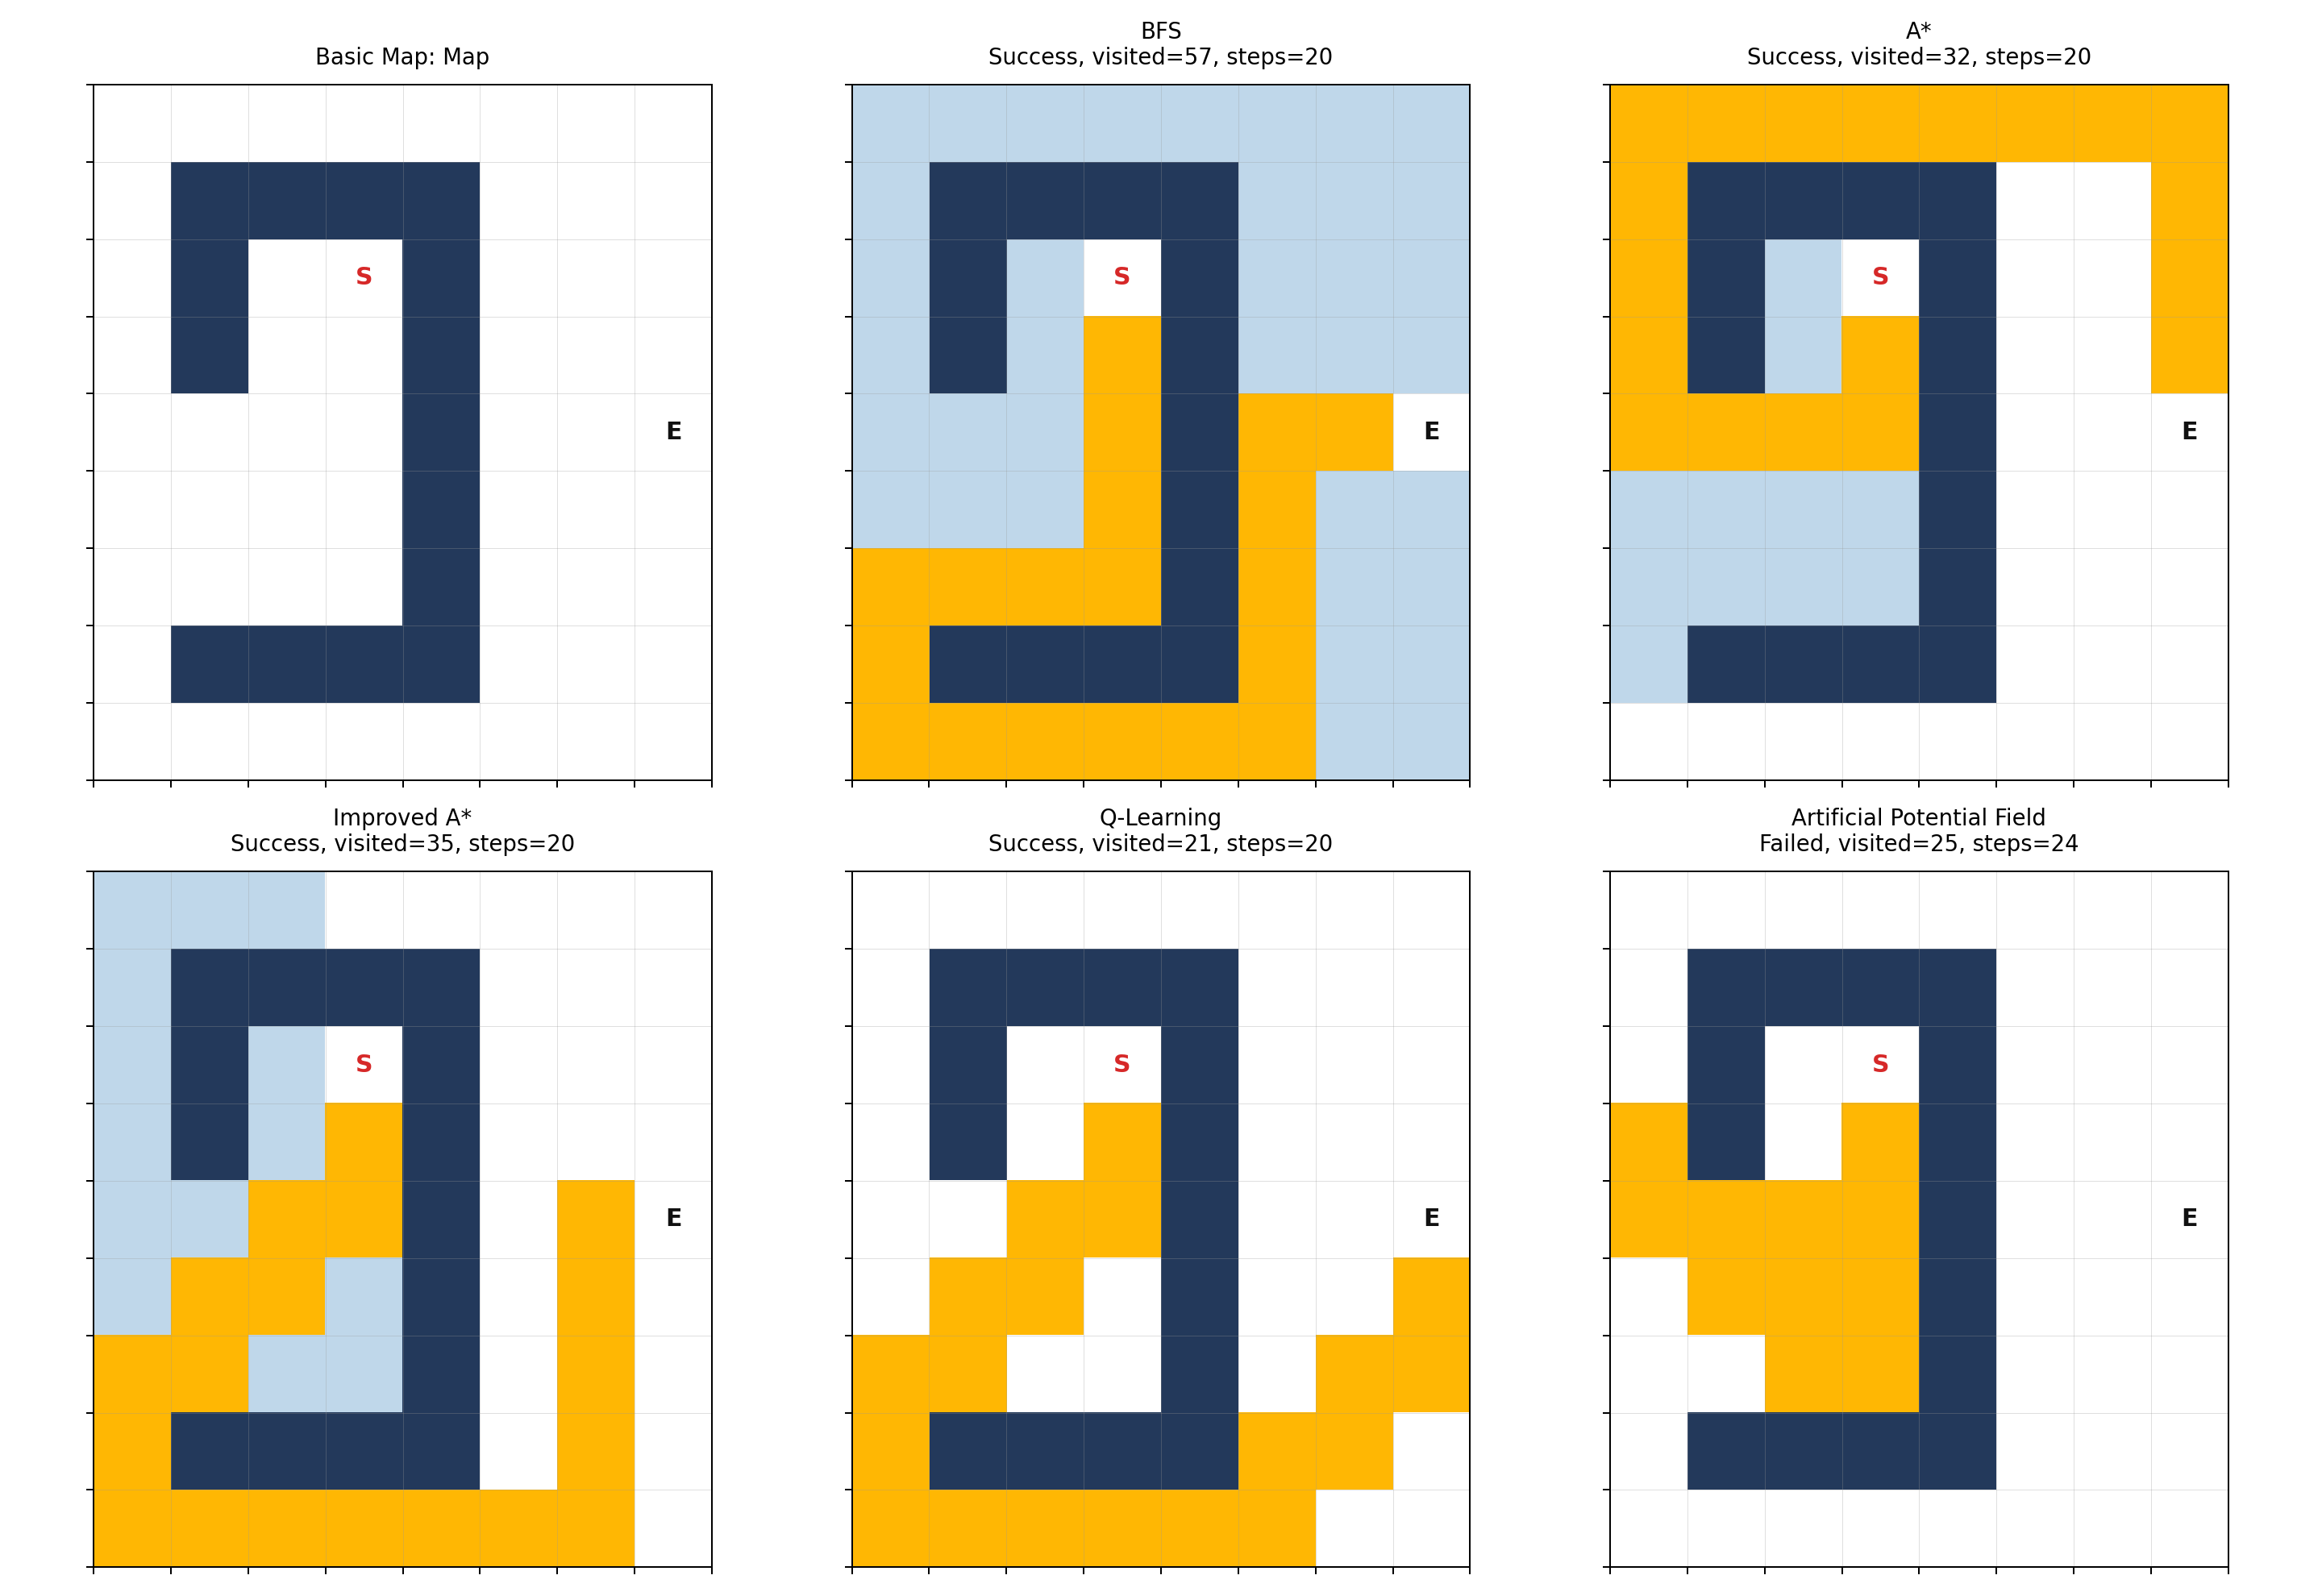
\includegraphics[width=0.85\textwidth]{../basic_map_comparison.png}
  \caption{基础场景下各算法结果对比}
  \label{fig:basic-comparison}
\end{figure}

\section{复杂场景结果}

在自主设计的 30$\times$30 复杂场景中，不同算法表现出更明显差异，如\cref{tab:challenge-result} 所示。

\begin{table}[!htb]
  \centering
  \caption{30x30 复杂场景实验结果}\label{tab:challenge-result}
  \begin{tabular}{@{}lcccc@{}}
    \toprule
    \textbf{算法} & \textbf{是否成功} & \textbf{访问节点数} & \textbf{路径步数} & \textbf{综合代价} \\
    \midrule
    BFS & 是 & 334 & 64 & 64.00 \\
    Dijkstra & 是 & 334 & 64 & 82.20 \\
    A* & 是 & 231 & 64 & 81.96 \\
    改进 A* & 是 & 263 & 64 & 79.56 \\
    Q-Learning & 是 & 65 & 64 & 81.64 \\
    人工势场法 & 否 & 91 & 90 & -- \\
    \bottomrule
  \end{tabular}
\end{table}

\begin{figure}[!htb]
  \centering
  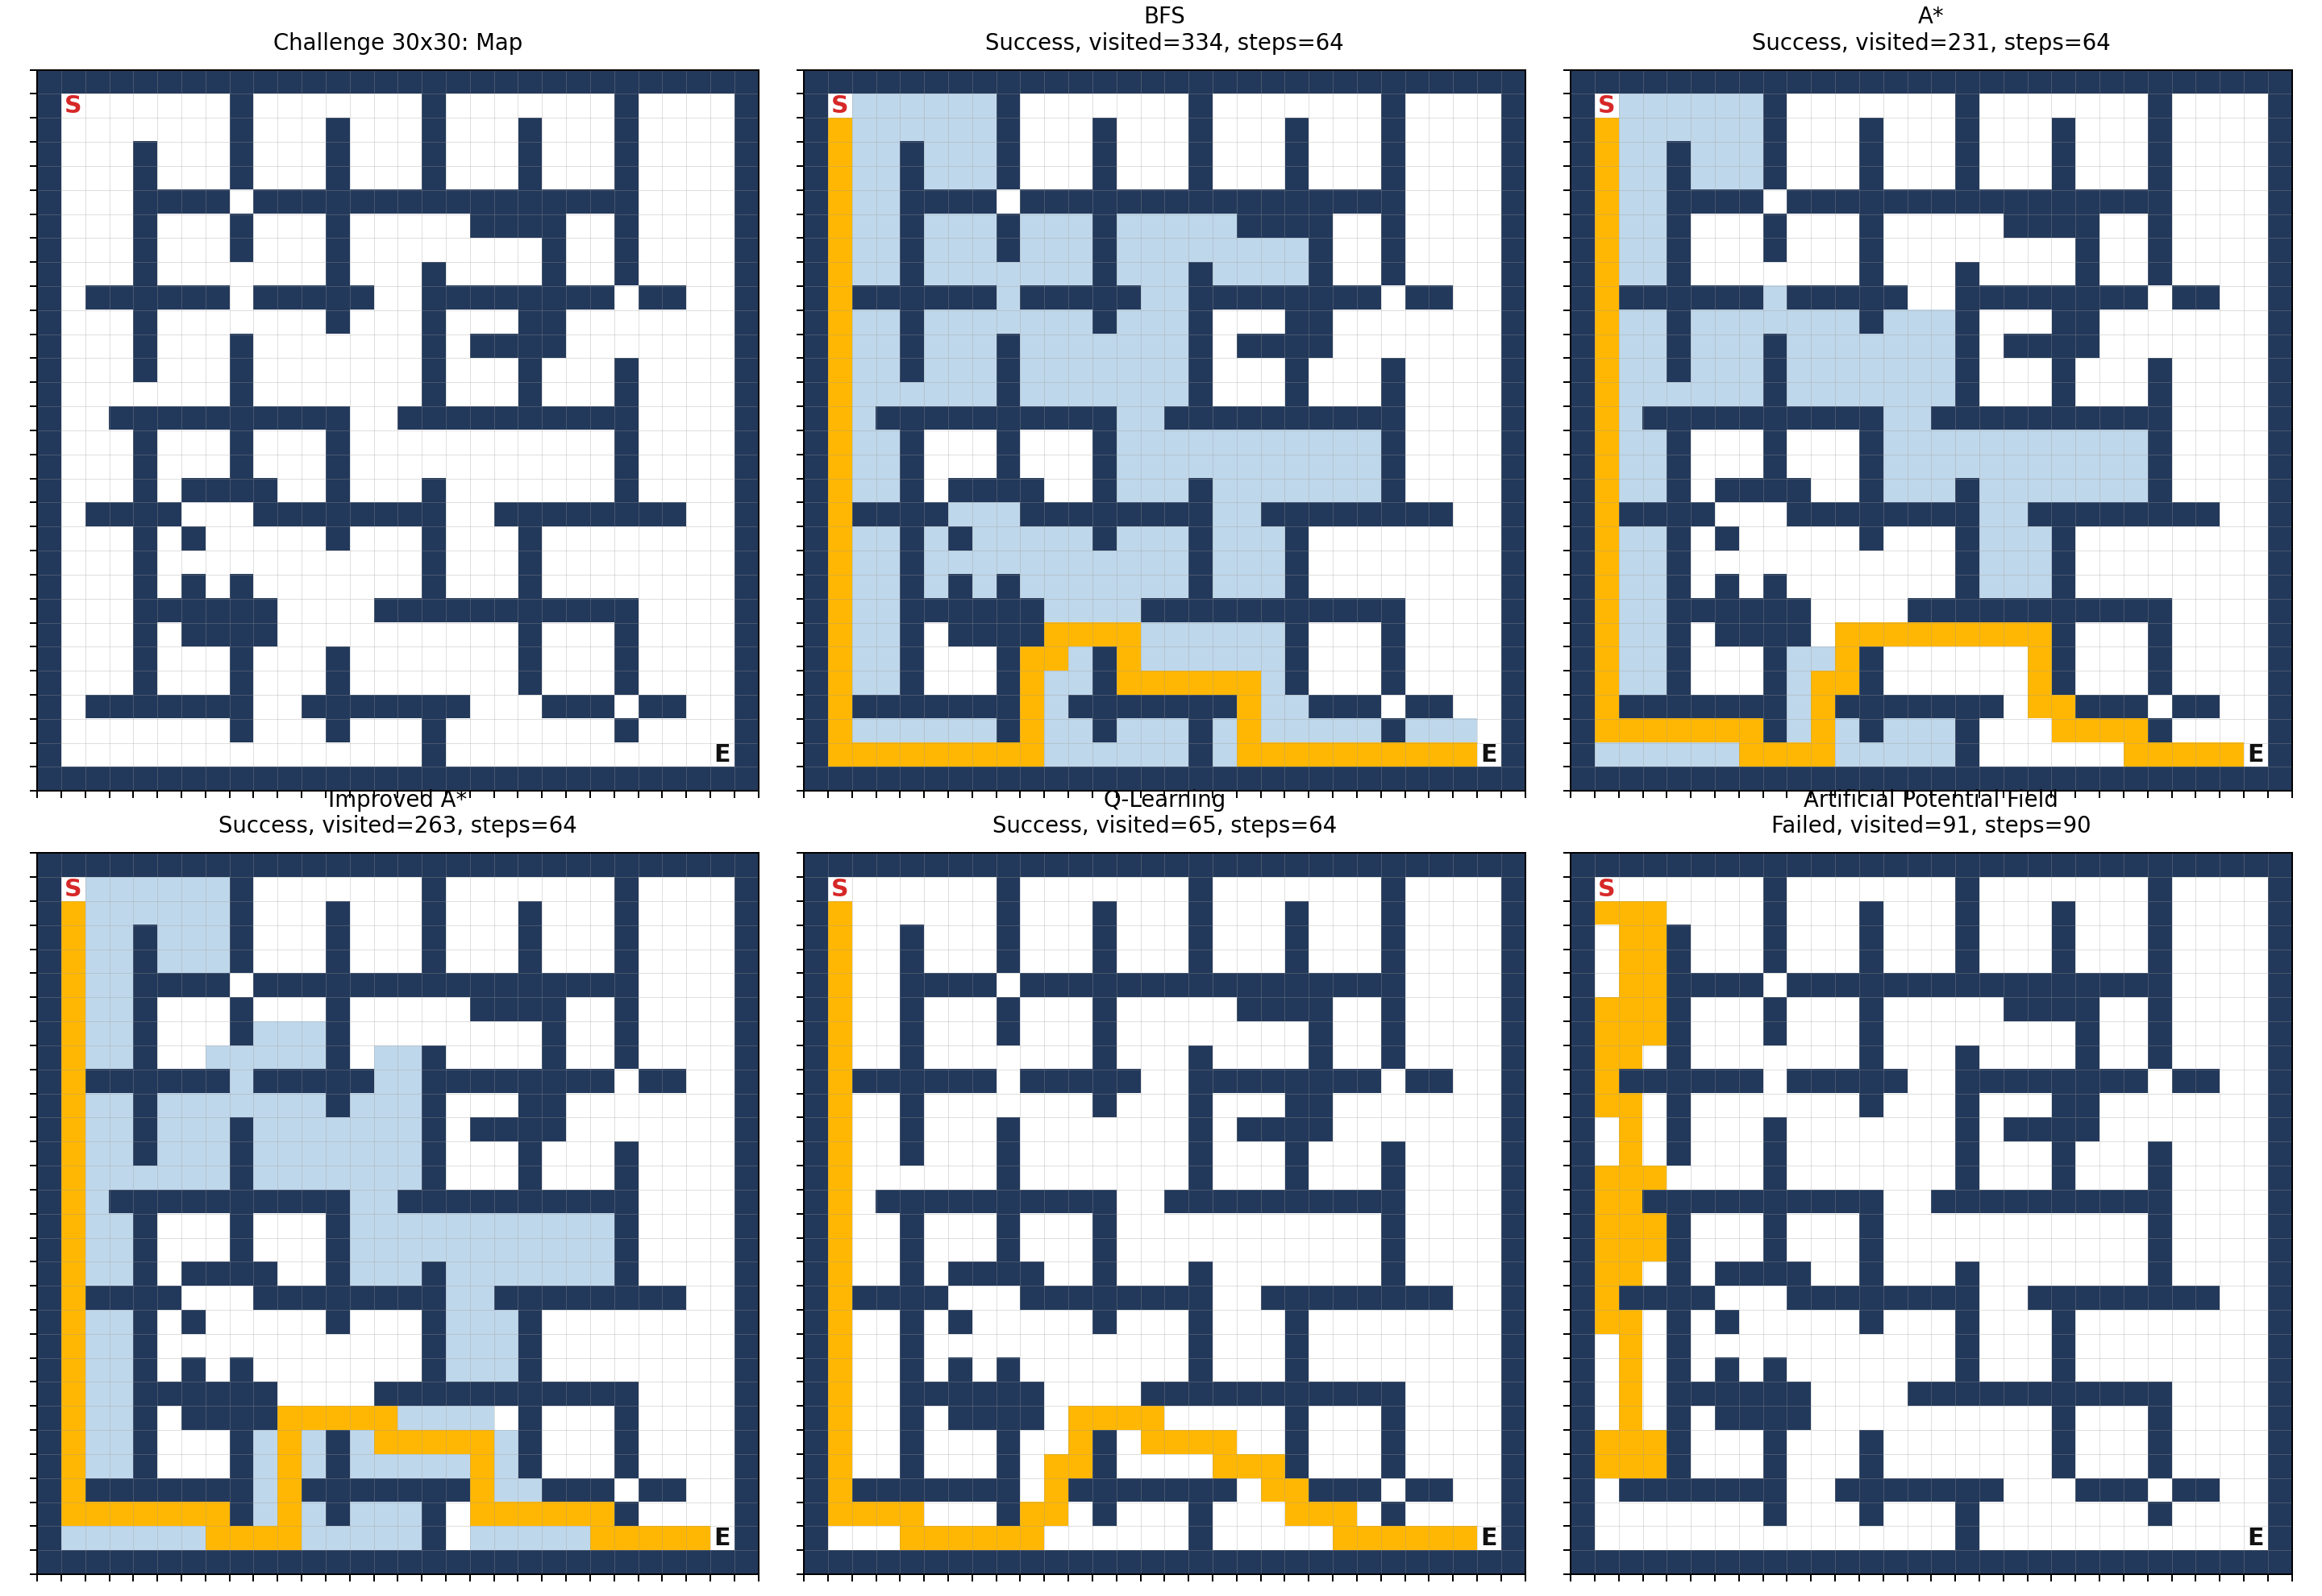
\includegraphics[width=0.93\textwidth]{../challenge_30x30_comparison.png}
  \caption{30x30 复杂场景下各算法结果对比}
  \label{fig:challenge-comparison}
\end{figure}

\begin{figure}[!htb]
  \centering
  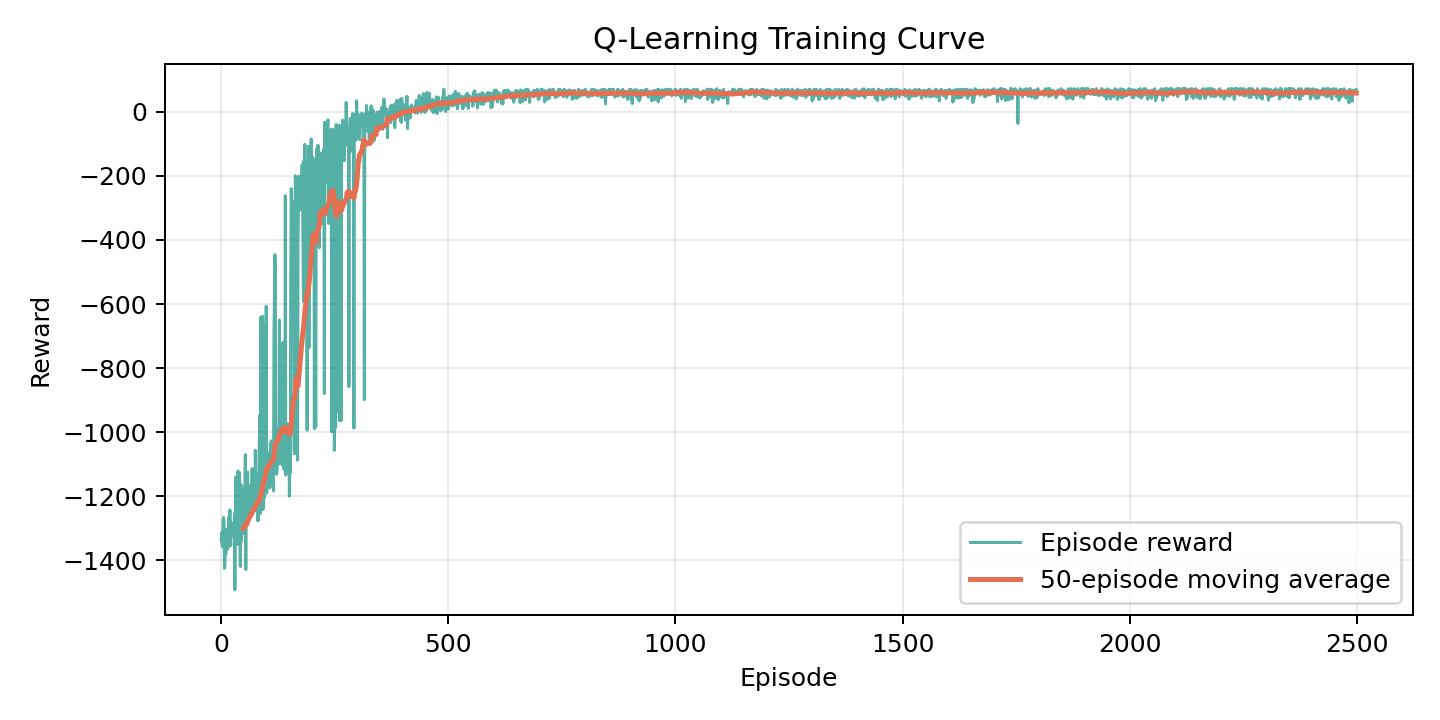
\includegraphics[width=0.72\textwidth]{../challenge_30x30_q_learning_curve.png}
  \caption{Q-Learning 在复杂场景中的训练回报曲线}
  \label{fig:qlearning-curve}
\end{figure}

\begin{figure}[!htb]
  \centering
  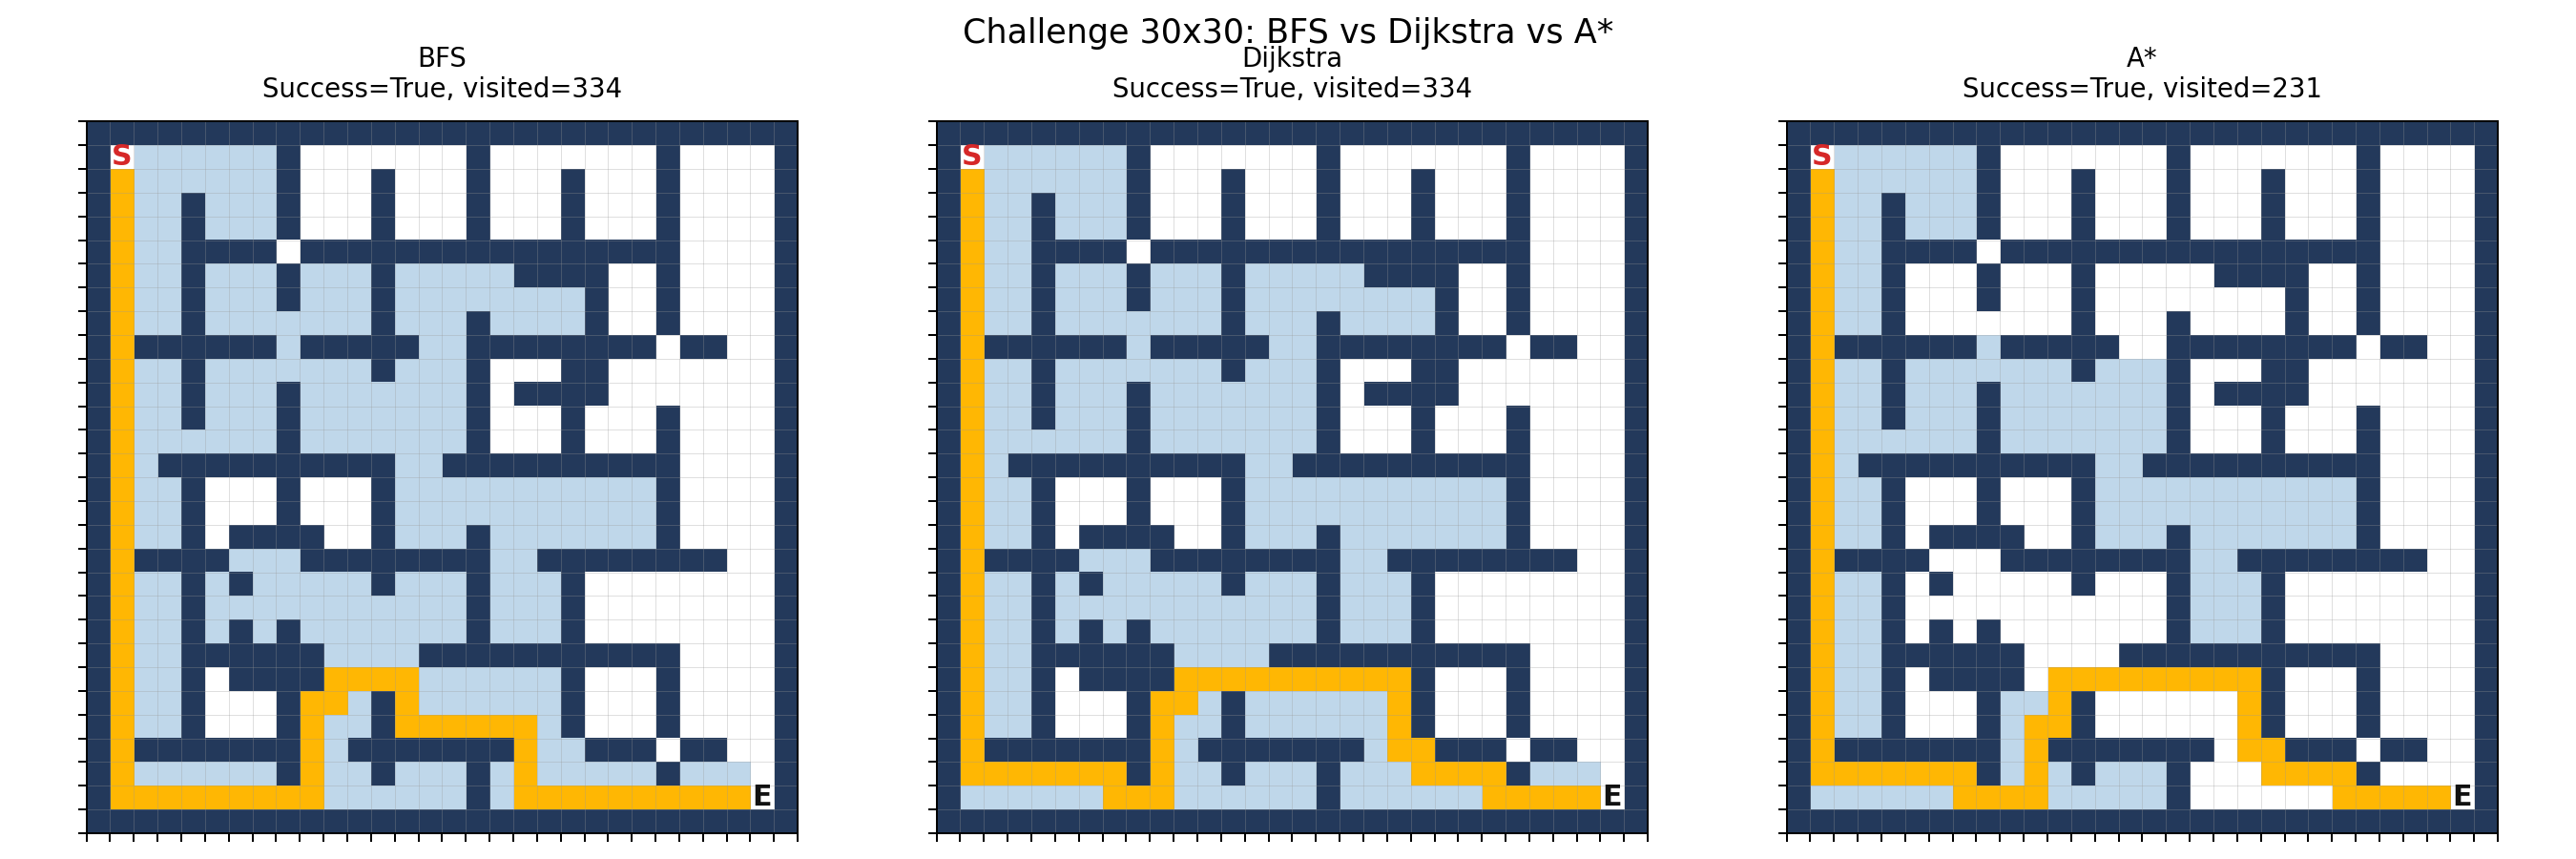
\includegraphics[width=0.78\textwidth]{../dijkstra_challenge_comparison.png}
  \caption{BFS、Dijkstra 与 A* 在复杂场景中的对比}
  \label{fig:dijkstra-comparison}
\end{figure}

\section{动态可视化结果}

为了满足题目对动态展示的要求，本文把 BFS、A* 和改进 A* 的搜索过程导出为 GIF 动画。整个动态展示分为两个阶段：

\begin{enumerate}
  \item 搜索阶段：按照节点访问顺序逐步显示已探索区域；
  \item 回溯阶段：在找到终点后逐步高亮最终路径。
\end{enumerate}

由于 PDF 不适合直接嵌入 GIF，这些动画作为随附文件提交。通过观察这些动态图，可以明显看出 BFS 的扩展更像“波纹式”铺开，而 A* 的搜索方向更集中，改进 A* 则更倾向于远离障碍区域。
